\begin{figure}[!htb]
	\centering
	\begin{subfigure}{0.45\textwidth}
		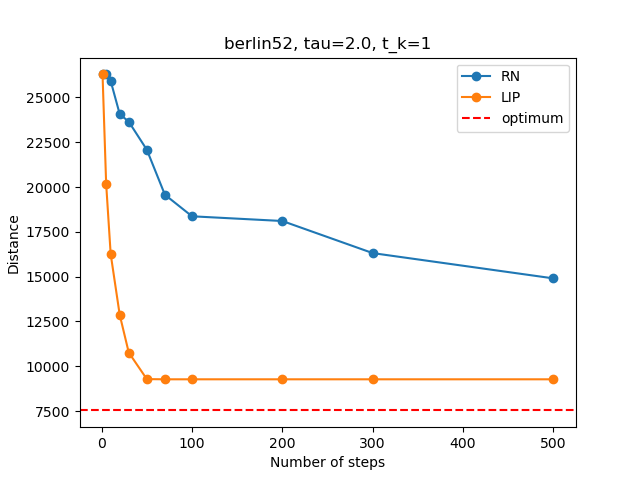
\includegraphics[width=\textwidth]{img/berlin52_temp=2.0_cool=1.0_low_iter}
		\subcaption{berlin52, $t_k=1$.}
	\end{subfigure}
	\begin{subfigure}{0.45\textwidth}
		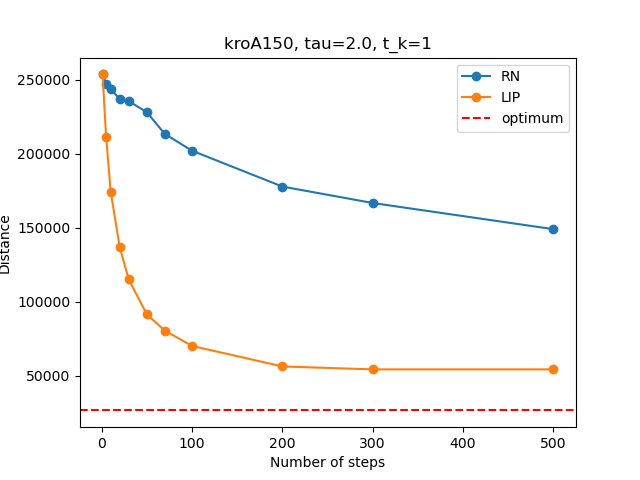
\includegraphics[width=\textwidth]{img/kroA150_temp=2.0_cool=1.0_low_iter}
		\subcaption{kroA150, $t_k=1$.}
	\end{subfigure}
	\caption{Comparing RN and LIP for \textit{berlin52} and \textit{kroA150} with low number of iterations.}
\end{figure}